% Chapter Template

\chapter{Results and Discussion} % Main chapter title

\label{Chapter5} % Change X to a consecutive number; for referencing this chapter elsewhere, use \ref{ChapterX}

\lhead{\emph{Results and Discussion}} % Change X to a consecutive number; this is for the header on each page - perhaps a shortened title

%----------------------------------------------------------------------------------------
%	SECTION 1
%----------------------------------------------------------------------------------------

The evaluation task is the most crucial step for a project. This section explains how this process is conducted then discuss the results. But first, let's take a look at the standard machine learning evaluations methods. 

\section{Machine learning evaluation methods}
In pattern recognition and information retrieval with binary classification usually a confusion matrix is used to evaluate the systems performance.
A confusion matrix \textit{(Kohavi and Provost, 1998)} contains information about actual and predicted classifications done by a classification system. Performance of such systems is commonly evaluated using the data in the matrix.
\begin{theorem}
\label{confusion matrix}
\emph{Confusion Matrix}

$$\bordermatrix{~ & political & non-political \cr
                  political & Tp & Fn \cr
                  non-political & Fp & Tn \cr}$$
\end{theorem}
Where:
\begin{itemize}
\item $Tp$ (True positive): is the number of \textbf{correct} predictions that an instance is political.
\item $Fn$  (False negative): is the number of \textbf{incorrect} predictions that an instance is non-political.
\item $Fp$ (False positive): is the number of \textbf{incorrect} of predictions that an instance political.
\item $Tn$ (True negative): is the number of \textbf{correct} predictions that an instance is non-political.
\end{itemize}                  

From the Confusion Matrix \ref{confusion matrix}, different evaluation patterns are extracted:
\begin{equation}
\label{eq:accuracy}
Accuracy = \frac{Tp+Tn}{Tp+Tn+Fp+Fn}
\end{equation}
\begin{equation}
\label{eq:precision}
Precision = \frac{Tp}{Tp+Fp}
\end{equation}
\begin{equation}
\label{eq:recall}
Recall = \frac{Tp}{Tp+Fn}
\end{equation}
\begin{equation}
\label{eq:fmeasure}
F_1 = 2.\frac{precision . recall}{precision+recall} = \frac{2Tp}{2Tp+Fp+Fn}
\end{equation}


To balance the influence between precision and recall in
traditional text classification, we will adopt the $F_1$-Measure\ref{eq:fmeasure} as our precision's criterion to evaluate the performance of the classifiers in a
global aspect.


\section{Evaluation and Results}
First, the corpus is divided into a \emph{test set} and a \emph{training set} where the size of each one is respectively $ \frac{3}{4}.corpus$ and $ \frac{1}{4}.corpus$.

Then to model a real life situation the features are extracted only from the training set.




The evaluation aim is to answer the following questions: combine the following criterion to get the best classification settings:
\begin{itemize}
\item What is the optimal number of features for a classifier?\\
As the Maximum Entropy classifier needs a lot of time to learn, the maximum number of feature tested is capped at 200.
\item How does the different machine learning algorithms perform?
\item What is the best feature engineering pattern ?
\end{itemize}

The following sections will answer the above questions. In addition for further testing and manipulations, the python code is available in the \textbf{evaluation.py} file.


\subsection{Unigram feature}


Special patterns features\ref{sec:special_patterns} (hashtags and names) are extracted using the \emph{PatternsFeatures()} class in the \textbf{feature\_extraction.py} file. The 10 most frequent names and hashtags are taken. They are added to the bag of word feature set.
The results of the next subsections can be reproduced by running the \emph{unigram\_evaluation(lines)} function in the  \textbf{evaluation.py} file.\\
\subsubsection{Frequency distribution}
Figure \ref{fig:fd_eval} shows the results of the evaluation using the Frequency distribution\ref{sec:fd} feature selection. In fact, we can see that the $F_1$-Measure of the algorithms are relatively close for a certain number of features. Table \ref{tab:fd_results} summarizes the results.

\begin{table}[H]
\begin{tabular}{c|c|c}
~ & max f-measure & number of features \\
Naive Bayes		&			 0.891013 		&		190\\
Maximum entropy		&		 0.893058 		&		70\\
Support Vector Machine	&	 0.900000 		&		110\\
\end{tabular}
\caption{Best algorithms results using Frequency Distribution}\label{tab:fd_results}
\end{table}



\begin{figure}[H]
  \centering
  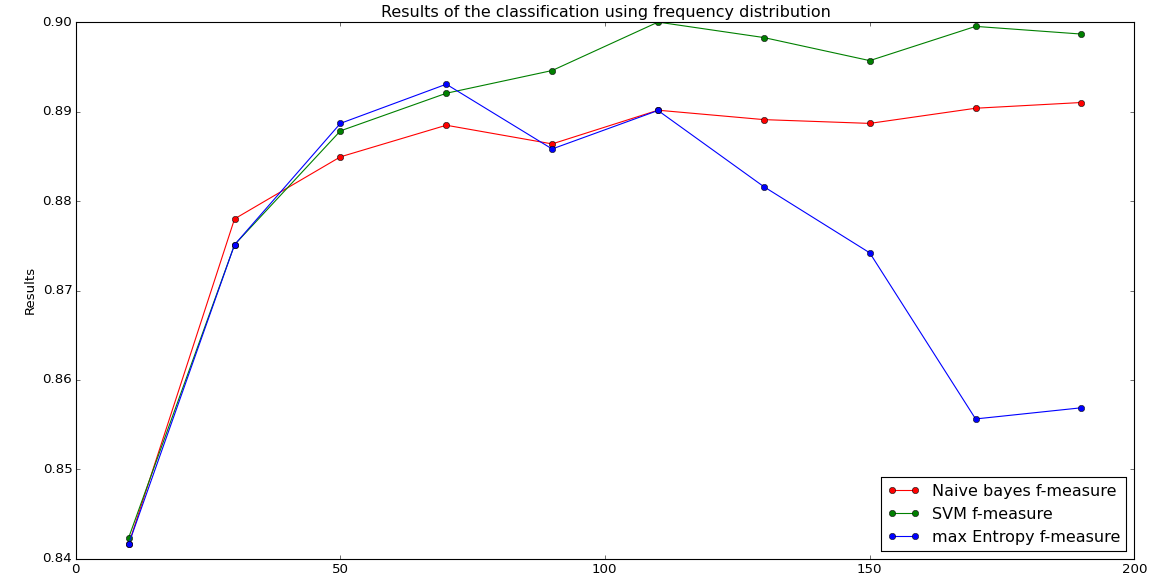
\includegraphics[width=160mm]{figures/result_fd_graph.png}
  \caption{Frequency Distribution Unigram F-Measure results for different number of features \label{fig:fd_eval}}
\end{figure}



\subsubsection{TF-IDF evaluation}
Figure \ref{fig:tfidf_eval} shows the results of the evaluation using the TF-IDF\ref{sec:tfidf} feature selection. In fact, we can see that the $F_1$-Measure of the algorithms are relatively close for a certain number of features. Table \ref{tab:tf-idf_results} summarizes the results.

\begin{table}[H]
\begin{tabular}{c|c|c}
		~	&				max f-measure 	& number of features \\
Naive Bayes			&		 0.894837 	&			190\\
Maximum entropy		&		 0.892791 	&			90\\
Support Vector Machine	&	 0.904215 	&			190\\
\end{tabular}
\caption{Best algorithms results using TF-IDF \label{tab:tf-idf_results}}
\end{table}

\begin{figure}[H]
  \centering
  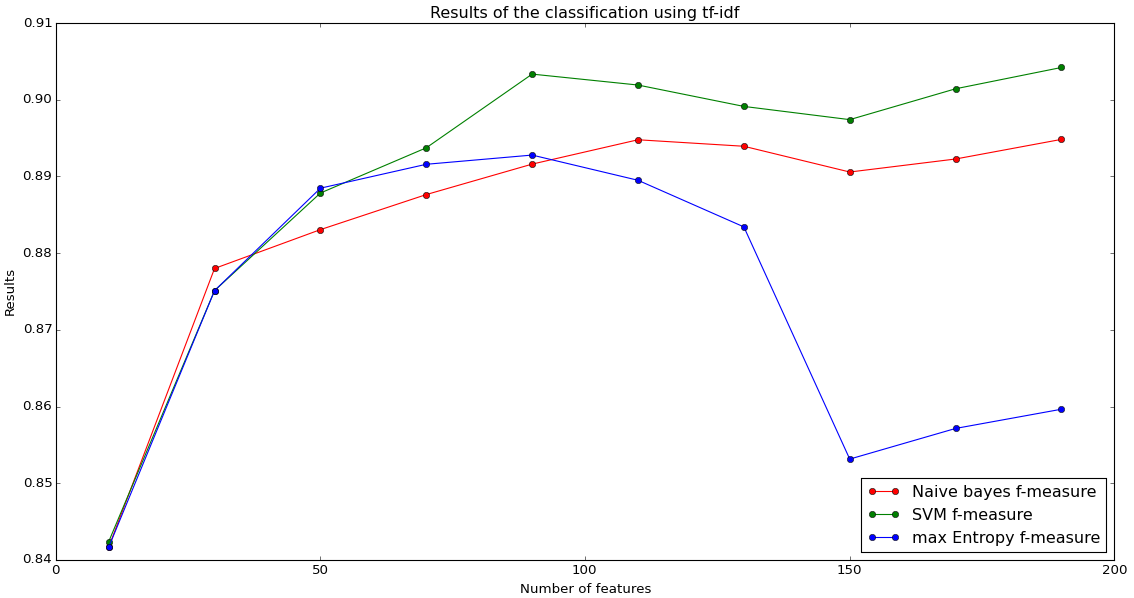
\includegraphics[width=160mm]{figures/result_tfidf_graph.png}
  \caption{tf-idf unigram F-Measure results for different number of features \label{fig:tfidf_eval}}
\end{figure}




\subsection{Bigram features}
\label{sec:bigram_results}
Figure \ref{fig:bigram_eval} shows that results of Bigram\ref{sec:bigram} features are constant. To have a better explanation of the result, the accuracy has been taken as well as the $F_1$-Measure. Table \ref{tab:tf-idf_results} summarizes the results.

\begin{table}[H]
\begin{tabular}{c|c|c}
		~	&				max f-measure 	& number of features \\
Naive Bayes			&		 0.754170 			&	170\\
Maximum entropy		&		 0.752347 			&	170\\
Support Vector Machine	&	 0.753623 			&	170\\
\end{tabular}
\caption{Best algorithms results using Frequency Distribution}\label{tab:bigram_results}
\end{table}


\begin{figure}[H]
  \centering
  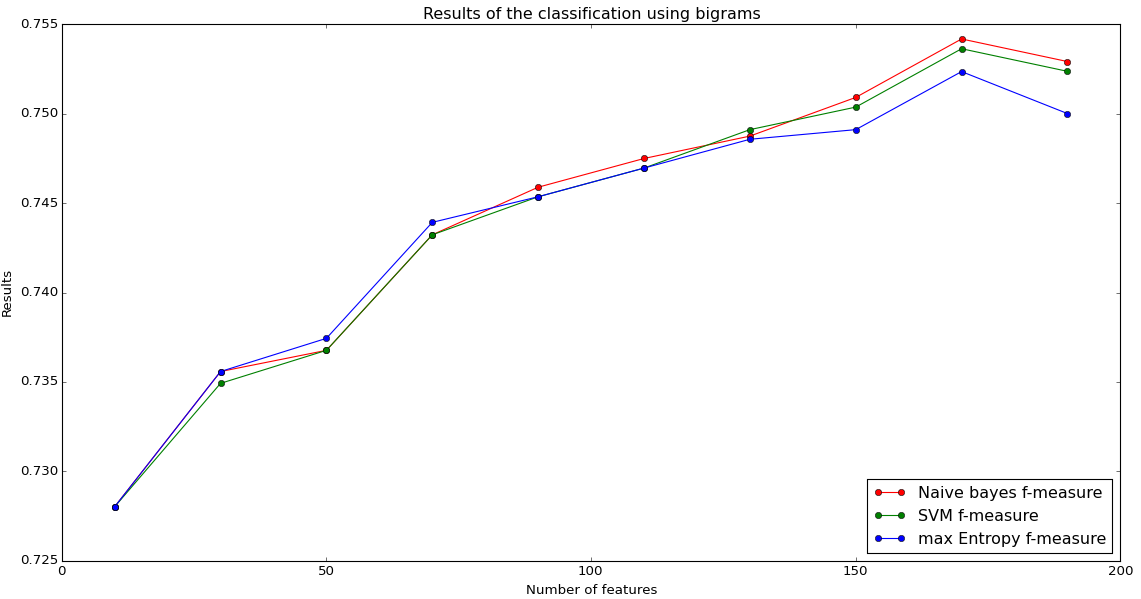
\includegraphics[width=160mm]{figures/bigram_results_graph.png}
  \caption{Bigrams F-Measure results for different number of features \label{fig:bigram_eval}}
\end{figure}

The results of this section can be reproduced by running the \emph{bigram\_evaluation(lines)} function in the  \textbf{evaluation.py} file.\\

\subsection{Combination of Unigrams and Bigrams }
\label{sec:combined_results}
The results shown in section \ref{sec:bigram_results} inform us that the overall outcome is independent from the number of bigrams used. At this end, only the 20 most frequent bigrams are used for this section.\\
Figure \ref{fig:uni_bi_eval} shows the results of the evaluation using Bigrams and Frequency Distribution feature selection. Table \ref{tab:tf-idf_results} summarizes the results.


\begin{table}[H]
\begin{tabular}{c|c|c}
		~	&				max f-measure 	& number of features \\
Naive Bayes				&	 0.818182 		&		190\\
Maximum entropy			&	 0.812893 		&		150\\
Suport Vector Machine	&	 0.824576 		&		200\\
\end{tabular}
\caption{Best algorithms results using Unigrams and Bigrams \label{tab:uni_bi_results}}
\end{table}

\begin{figure}[H]
  \centering
  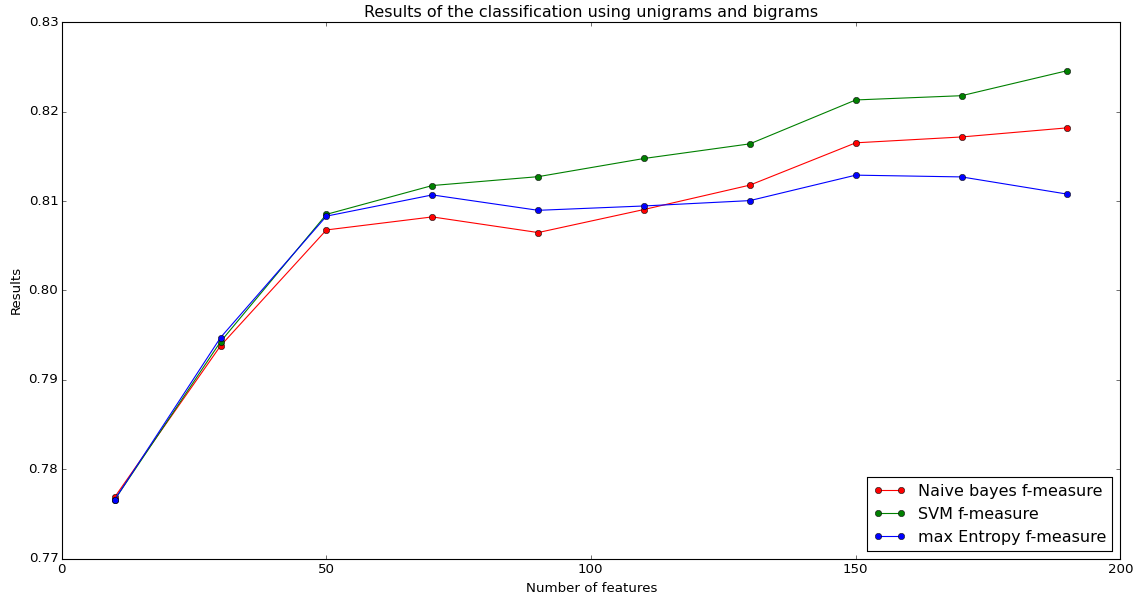
\includegraphics[width=160mm]{figures/combination_graph.png}
  \caption{Combination of Unigrams and Bigrams F-Measure results for different number of features \label{fig:uni_bi_eval}}
\end{figure}


The results of this section can be reproduced by running the \emph{uni\_and\_bi\_evaluation(lines)} function in the  \textbf{evaluation.py} file.\\

\section{Discussions}
\subsection{Result discussion}
The $F_1$-Measure results are relatively close in each test case. We can see that the Support Vector Machine classifier has a slight edge.\\
The unigram classification test the results show that the Support Vector Machine and Naïve Bayes classifiers reaches their best $F_1$-Measure for 190 features. This is an expected result because of the nature of these classifiers. However the maximum entropy falls down in $F_1$-Measure after reaching a peak at 70 features. This is explained by the motivation behind maximum entropy. In fact it says that one should prefer the most uniform models that satisfy any given constraint. By adding more features, the maximum entropy classifier needs more iterations to reach the best results. In this work the number of iterations for the Maximum Entropy classifier is 100 as it takes a lot of computation time.\\
The bigram classification test the results display an inferior result comparing to the unigram findings. This is explained by the frequency of a bigram. In fact the frequency  is very low compared to the unigrams.\\
This can be verified by running the next code.
\begin{lstlisting}[language=Python]
import preprocess
from nltk import FreqDist, bigrams
filename = "all_tweets.txt"
lines = preprocess.main(filename) 
all_tweets = " ".join([" ".join(line[1]) for line in lines])
print " 10 most frequent bigrams", FreqDist(bigrams(all_tweets.split(" "))).most_common(10)
print " 10 most frequent unigrams", FreqDist(all_tweets.split(" ")).most_common(10)
\end{lstlisting}
The outcome of the code of shown above reveal that the most frequent bigram appears 55 times although the most frequent unigram appears 429 times.
\begin{lstlisting}[language=Python]
10 most frequent bigrams  [((u'health', u'care'), 55), ((u'sarah', u'palin'), 37), ((u'president', u'obama'), 28), ((u'barack', u'obama'), 22), ((u'white', u'house'), 16), ((u'care', u'reform'), 16), ((u'bill', u'clinton'), 16), ((u'#tcot', u'#tlot'), 16), ((u'pres', u'obama'), 13), ((u'blog', u'post'), 13)]
 10 most frequent unigrams  [(u'obama', 433), (u'government', 260), (u'economy', 177), (u'afghanistan', 126), (u'2', 120), (u'good', 117), (u'senate', 115), (u'#tcot', 114), (u'congress', 110), (u'lol', 104)]
\end{lstlisting}

Finally, the combination of unigrams and bigrams has a fair result but not as good as unigram alone.
 
\subsection{Limitations}
The data set was collected between June 1, 2009 and Dec 31, 2009. The political subjects are dynamic and topics, key words change often. Therefor this model can't classify real time tweets.\\
Moreover this classification model works only on English tweets.\\
The special patterns features are limited since more than 50\% of the tweets does not contain a hashtag or/ and name.
\subsection{Improvements}
This project work can be improved, these are some ways:
\begin{itemize}
\item Test unsupervised learning algorithms.
\item Try to fetch new political tweets to keep the corpora up to date.
\end{itemize}
